\chapter{Pääluvun otsikko}

\section{Alaluvun otsikko}
Otsikon jälkeen tulee tekstiä tai uusi alaotsikko. Kuvien alapuolelle ja taulukkojen yläpuolelle tulee numero, seloste ja tarvittaessa lähdeviite.

Kuva merkitään Kuva-tyylin mukaiseksi; tämä on tarpeen, jottei kuvan ja sen otsikon väliin voi tulla sivunvaihtoa. Kuvan selite merkitään Kuvan selite -tyylin mukaiseksi. Tällöin kuvat numeroituvat automaattisesti.

\begin{figure}[h]
  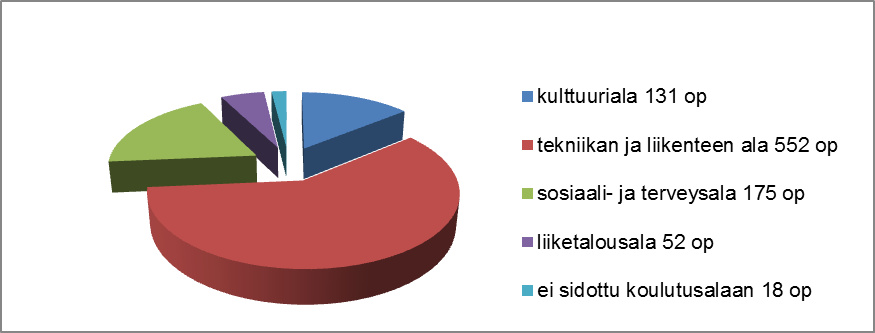
\includegraphics[width=\textwidth]{chart}
  \caption{Metropolian opiskelijoiden lukuvuonna 2009–2010 suorittamat virtuaaliopinnot. Virtuaaliopintojen määrä on ilmaistu opintopisteinä (op).}
  \label{fig:chart}
\end{figure}

Tarjolla on myös tyylit Kuvio ja Kuvion selite. Ainoana erona on se, että selitetekstiin tulostuu tällöin sana ”Kuvio”.

Kuvan tai taulukon jälkeen tulee tekstiä ennen uutta kuvaa tai taulukkoa tai seuraavaa otsikkoa.

\section{Alaluvun otsikko}

\subsection{Alaluvun alaotsikko}

Otsikon jälkeen tulee tekstiä tai uusi alaotsikko.

\begin{table}[h]
  \caption{Metropolian opiskelijoiden lukuvuonna 2009–2010 suorittamat virtuaaliopinnot.}
  \begin{tabular}{| l | l | l |}
  \hline
  \bfseries Koulutusala & \bfseries Suoritusten määrä, op \\
  \hline
  Kulttuuriala & 131 \\
  \hline
  Tekniikan ja liikenteen ala & 552 \\
  \hline
  Sosiaali- ja terveysala & 175 \\
  \hline
  Liiketaloudena ala & 52 \\
  \hline
  Ei sidottu koulutusalaan & 18 \\
  \hline
  \bfseries Metropolia yhteensä & \bfseries 928 \\
  \hline
  \end{tabular}
  \label{tab:virtual studies}
\end{table}

Kuvan tai taulukon jälkeen tulee tekstiä ennen uutta kuvaa tai taulukkoa tai seuraavaa otsikkoa.

\subsection{Alaluvun alaotsikko}

Alaluvun alaotsikon jälkeen tulee tekstiä.

Sitaatti toteutetaan Lainaus-tyylillä. Sitaatin johtolauseen sisältävässä kappaleessa (välittömästi sitaattia edeltävässä kappaleessa) käytetään tyyliä ”Leipäteksti ennen lainausta”, jotta sitaatin ja johtolauseen väliin jää lyhyempi kappaleväli.

\begin{quote}
Usean rivin pituinen suora lainaus kirjoitetaan kirjainkoolla 10. Tekstissä käytetään riviväliä 1, ja teksti sisennetään. Suorassa lainauksessa käytetään mallipohjan lainaustyyliä. Lainaukseen merkitään lähdeviite.
\end{quote}

Teksti jatkuu sisennyksen jälkeen vasemmasta reunasta leipätekstityylillä.

Tekstissä oleva luetelma toteutetaan luetelmatyylillä:

\begin{bullet-list}
  \item Tämä on luetelman ensimmäinen kohta.
  \item Toinen luetelman kohta sisältää tässä pitkän tekstin, joka ulottuu monelle riville. Vasen reuna tasautuu automaattisesti.
  \item Tämä on luetelman kolmas kohta.
  \item Luetelman neljäs kohta on tässä.
\end{bullet-list}

Luetelman osat kirjoitetaan isolla kirjaimella ja jokaisen jälkeen pannaan piste, kun luetelma koostuu kokonaisista lauseista.

Luetelman osat alkavat pienellä kirjaimella ja viimeisen osan perään tulee piste, kun osat eivät ole lauseita. Insinöörityö koostuu

\begin{bullet-list}
  \item sanoista
  \item lauseista
  \item virkkeistä
  \item kappaleista
  \item luvuista.
\end{bullet-list}

Teksti jatkuu luetelman jälkeen vasemmasta reunasta leipätekstityylillä.

Insinöörityöhön voidaan liittää omalla rivillään esitettyjä, numeroituja kaavoja:

\begin{equation}
  x = \frac{-b \pm \sqrt{b^{2} - 4ac}}{2a}
\end{equation}

Lisää uusi kaava valitsemalla Lisää/Pikaosat/Kaava kaavatoiminnolla. Jos haluat käyttää kaavatoiminnon sijasta vanhaa kaavaeditoria, valitse Lisää/Pikaosat/Kaava (MS Kaava 3.0 -objektina).